
Software projects, either directly or indirectly, span multiple code repositories. Dealing with local project code is the easiest, but software projects are rarely standalone. Things may get complicated really fast without a proper dependency management strategy. The first recommendation of this chapter is to use a package manager if you can. Package managers greatly reduce the effort spent on dependency management. If you are not able to use a package manager, you may need to roll your very own mini project-specific package manager, which is called a super-build.

Super-builds are mostly used for making a project self-sufficient dependency-wise, which means the project is able to satisfy its very own dependencies without the intervention of the user. Having such an ability is very convenient for all consumers. To demonstrate this technique, we will start with an example of such a scenario. Let's begin.


\subsubsubsection{10.3.1\hspace{0.2cm}The recommended way – FetchContent}

We will be following Chapter 10, Example 01 for this part. Let's start by inspecting Chapter 10, Example 01's CMakeLists.txt file, as usual. The first seven lines are left out for simplicity:

\begin{lstlisting}[style=styleCMake]
if(CH10_EX01_USE_SUPERBUILD)
	include(superbuild.cmake)
else()
	find_package(GTest 1.10.0 REQUIRED)
	find_package(benchmark 1.6.1 REQUIRED)
endif()

add_executable(ch10_ex01_tests)
target_sources(ch10_ex01_tests PRIVATE src/tests.cpp)
target_link_libraries(ch10_ex01_tests PRIVATE GTest::Main)

add_executable(ch10_ex01_benchmarks)
target_sources(ch10_ex01_benchmarks PRIVATE src
	/benchmarks.cpp)
target_link_libraries(ch10_ex01_benchmarks PRIVATE
	benchmark::benchmark)
\end{lstlisting}

As we can see, it is a simple CMakeLists.txt file that defines two targets, named ch10\_ex01\_tests and ch10\_ex01\_benchmarks. These targets depend on Google Test and Google Benchmark libraries, respectively. These libraries are found and defined by either the super-build or the find\_package(…) calls, depending on the CH10\_EX01\_USE\_SUPERBUILD variable. The find\_package(…) path is the way we have followed until now. Let's inspect the super-build file, superbuild.cmake, together:

\begin{lstlisting}[style=styleCMake]
include(FetchContent)
FetchContent_Declare(benchmark
	GIT_REPOSITORY https://github.com/google/benchmark.git
	GIT_TAG v1.6.1
)
FetchContent_Declare(GTest
	GIT_REPOSITORY https://github.com/google/googletest.git
	GIT_TAG release-1.10.0
)
FetchContent_MakeAvailable(GTest benchmark)
add_library(GTest::Main ALIAS gtest_main)
\end{lstlisting}

In the first line, the FetchContent CMake module is included, since we are going to utilize it for the dependencies. In the following six lines, the FetchContent\_Declare function is used to declare two external targets, benchmark and GTest, which are instructed to be fetched via Git. Consequently, the FetchContent\_MakeAvailable(…) function is called to make the declared targets available. Lastly, an add\_library(…) call is made for defining an alias target named GTest::Main for the gtest\_main target. This is done to keep the compatibility between find\_package(…) and super-build target names. There is no alias target defined for benchmark, since its find\_package(…) and super-build target names are already compatible.

Let's configure and build the example by invoking the following commands:

\begin{tcblisting}{commandshell={}}
cd chapter_10/ex01_external_deps
cmake -S ./ -B build -DCH10_EX01_USE_SUPERBUILD:BOOL=ON
cmake --build build/ --parallel $(nproc)
\end{tcblisting}

In the first two lines, we are going into the example\_10/ folder and configuring the project. Note that we are setting the CH10\_EX01\_USE\_SUPERBUILD variable to ON in order to enable the super-build code. In the last line, we are building the project with N parallel jobs, where N is the result of the nproc command.
 
Thanks to the alternate find\_package(...) path, the build will also work fine without enabling the super-build, given that google test >= 1.10.0 and google benchmark >= 1.6.1 are available in the environment. This will allow package maintainers to change dependency versions without patching the project. Small customization points such as this are important for portability and reproducibility.

Up next, we'll be taking a look at a super-build example that uses the ExternalProject module instead of the FetchContent module.

\subsubsubsection{10.3.2\hspace{0.2cm}The legacy way – ExternalProject\_Add}

Before FetchContent was a thing, most people implemented the super-build approach by utilizing the ExternalProject\_Add CMake function. This function is provided by the ExternalProject CMake module. In this section, we will see a superbuild example with ExternalProject\_Add to see how it differs from using the FetchContent module.

Let's take a look at the CMakeLists.txt file in Chapter 10, Example 02 together (comments and the project directive are omitted):

\begin{lstlisting}[style=styleCMake]
# ...
include(superbuild.cmake)
add_executable(ch10_ex02_tests)
target_sources(ch10_ex02_tests PRIVATE src/tests.cpp)
target_link_libraries(ch10_ex02_tests PRIVATE catch2)
\end{lstlisting}

Again, the project is a unit-test project containing a single C++ source file, but this time it is with Catch2 instead of Google Test. The CMakeLists.txt file includes the superbuild.cmake file directly, defines an executable target, and links the Catch2 library to the target. You may have noticed that this example does not use FindPackage(...) to discover the Catch2 library. The reason for this is that, unlike FetchContent, ExternalProject fetches and builds the external dependencies at build time. Since the content of the Catch2 library is not available at configuration time, we are unable to use FindPackage(...) here. FindPackage(…) runs at configure time and requires the package files to be present. Let's take a look at superbuild.cmake as well:

\begin{lstlisting}[style=styleCMake]
include(ExternalProject)
ExternalProject_Add(catch2_download
	GIT_REPOSITORY https://github.com/catchorg/Catch2.git
	GIT_TAG v2.13.9
	INSTALL_COMMAND ""
	# For disabling the warning that treated as an error
	CMAKE_ARGS -DCMAKE_CXX_FLAGS="-Wno-error=pragmas"
)
SET(CATCH2_INCLUDE_DIR ${CMAKE_CURRENT_BINARY_DIR}
	/catch2_download-prefix/src/catch2_download/single_include)
file(MAKE_DIRECTORY ${CATCH2_INCLUDE_DIR})
add_library(catch2 IMPORTED INTERFACE GLOBAL)
add_dependencies(catch2 catch2_download)
set_target_properties(catch2 PROPERTIES "INTERFACE_INCLUDE_
	DIRECTORIES" "${CATCH2_INCLUDE_DIR}")
\end{lstlisting}

The superbuild.cmake module includes the ExternalProject CMake module. The code calls the ExternalProject\_Add function to declare a target named catch2\_download with the GIT\_REPOSITORY, GIT\_TAG, INSTALL\_COMMAND, and CMAKE\_ARGS arguments. As you may recall from previous chapters, the ExternalProject\_Add function can fetch dependencies from different sources. Our example is trying to fetch the dependency via using Git. The GIT\_REPOSITORY and GIT\_TAG arguments are for specifying the target Git repository URL and the tag to be checked out after the git clone, respectively. Since Catch2 is a CMake project, the amount of parameters we need to supply to the ExternalProject\_Add function is minimal. The ExternalProject\_Add function knows how to configure, build, and install a CMake project by default, so no CONFIGURE\_COMMAND or BUILD\_COMMAND arguments are needed. The empty INSTALL\_COMMAND argument is for disabling and installing the dependency after the build. The last argument, CMAKE\_ARGS, is for passing CMake arguments to the external project's configure step. We use this to suppress a GCC warning (treated as an error) about legacy pragmas in the Catch2 compilation.

The ExternalProject\_Add command fetches the desired library into a prefix path and builds it. So, to use the fetched content, we have to import it to the project first. Since we cannot utilize FindPackage(...) to let CMake deal with the importing of the library, we have some manual work to do. One of them is to define the include directory of the Catch2 target. Since Catch2 is a header-only library, defining an interface target with the headers will be sufficient. We are declaring the CATCH2\_INCLUDE\_DIR variable to set the directory that will contain the Catch2 headers. We are using this variable to set the INTERFACE\_INCLUDE\_DIRECTORIES property of the imported target created in this example. Up next, the file (MAKE\_DIRECTORY \$\{CATCH2\_INCLUDE\_DIR\}) CMake command is called to create the include directory. The reason for that is, because of how ExternalProject\_Add works, the Catch2 content is not present until the build step executes. Setting a target's INTERFACE\_INCLUDE\_DIRECTORIES requires the given directories to be present, so we're doing a small hack as a workaround. In the last three lines, we declare an IMPORTED INTERFACE library for Catch2, making this library dependent on the catch2\_download target and setting INTERFACE\_INCLUDE\_DIRECTORIES of the imported library.

Let's try to configure and build our example to check whether it works or not:

\begin{tcblisting}{commandshell={}}
cd chapter_10/ex02_external_deps_with_extproject
cmake -S ./ -B build
cmake --build build/ --parallel $(nproc)
\end{tcblisting}

If everything goes as expected, you should be seeing output similar to this:

\begin{tcblisting}{commandshell={}}
[ 10%] Creating directories for 'catch2_download'
[ 20%] Performing download step (git clone) for
  'catch2_download'
Cloning into 'catch2_download'...
HEAD is now at 62fd6605 v2.13.9
[ 30%] Performing update step for 'catch2_download'
[ 40%] No patch step for 'catch2_download'
[ 50%] Performing configure step for 'catch2_download'
/* ... */
[ 60%] Performing build step for 'catch2_download'
/* ... */
[ 70%] No install step for 'catch2_download'
[ 80%] Completed 'catch2_download'
[ 80%] Built target catch2_download
/* ... */
[100%] Built target ch10_ex02_tests
\end{tcblisting}

Alright, it seems we have built our test executable successfully. Let's run it to check whether it works by running the ./build/ch10\_ex02\_tests executable:

\begin{tcblisting}{commandshell={}}
===========================================================
All tests passed (4 assertions in 1 test case)
\end{tcblisting}

Up next, we'll see a simple QT application using the QT framework from a super-build.

\subsubsubsection{10.3.3\hspace{0.2cm}Bonus – using the Qt 6 framework with a super-build}

Until now, we have dealt with libraries that have rather small footprints. Let's try something more complex, such as using a big framework such as the Qt framework in a super-build. For this part, we are going to follow the Chapter 10, Example 03 example.

\begin{tcolorbox}[colback=blue!5!white,colframe=blue!75!black,title=Important note]
If you are going to try this example outside of the provided Docker container, you may have to install some additional dependencies required by the Qt runtime. The required packages for the Debian-like systems are as follows: libgl1-mesa-dev libglu1-mesa-dev '\^{}libxcb.*-dev' libx11-xcb-dev libglu1-mesa-dev libxrender-dev libxi-dev libxkbcommon-dev libxkbcommon-x11-dev.
\end{tcolorbox}

The example contains a single source file, main.cpp, that outputs a simple Qt window application with a message. The implementation is as follows:

\begin{lstlisting}[style=styleCXX]
#include <qapplication.h>
#include <qpushbutton.h>
int main( int argc, char **argv )
{
	QApplication a( argc, argv );
	QPushButton hello( "Hello from CMake Best Practices!",
	0 );
	hello.resize( 250, 30 );
	hello.show();
	return a.exec();
}
\end{lstlisting}

Our goal is to be able to compile this Qt application without requiring the user to install the Qt framework themselves. The super-build should automatically install the Qt 6 framework, and the application should be able to use that. Let's take a look at the CMakeLists.txt file of the example, as usual:

\begin{lstlisting}[style=styleCMake]
if(CH10_EX03_USE_SUPERBUILD)
	include(superbuild.cmake)
else()
	set(CMAKE_AUTOMOC ON)
	set(CMAKE_AUTORCC ON)
	set(CMAKE_AUTOUIC ON)

	find_package(Qt6 COMPONENTS Core Widgets REQUIRED)
endif()
add_execu
table(ch10_ex03_simple_qt_app main.cpp)
target_compile_features(ch10_ex03_simple_qt_app PRIVATE
	cxx_std_11)
target_link_libraries(ch10_ex03_simple_qt_app Qt6::Core
	Qt6::Widgets)
\end{lstlisting}

Like the first example, the CMakeLists.txt file includes the superbuild.cmake file, depending on an option flag. If the user is opted in to use a super-build for the example, it will include the super-build module. Otherwise, the dependency will try to be located in the system via find\_package(...). In the last three lines, an executable target is defined, C++ standards for the target are set, and the defined target is linked to the QT6::Core and QT6::Widgets targets. These targets are either defined by the super-build or the find\_package(...) call, depending on whether the user is opted in to use the super-build or not. Let's continue by taking a look at the superbuild.cmake file:

\begin{lstlisting}[style=styleCMake]
include(FetchContent)
message(STATUS "Chapter 10, example 03 superbuild enabled.
	Will try to satisfy dependencies for the example.")
set(FETCHCONTENT_QUIET FALSE) # Enable message output for
	FetchContent commands
set(QT_BUILD_SUBMODULES "qtbase" CACHE STRING "Submodules
	to build")
set(QT_WILL_BUILD_TOOLS on)
set(QT_FEATURE_sql off)
set(QT_FEATURE_network off)
set(QT_FEATURE_dbus off)
set(QT_FEATURE_opengl off)
set(QT_FEATURE_testlib off)
set(QT_BUILD_STANDALONE_TESTS off)
set(QT_BUILD_EXAMPLES off)
set(QT_BUILD_TESTS off)

FetchContent_Declare(qt6
	GIT_REPOSITORY https://github.com/qt/qt5.git
	GIT_TAG v6.3.0
	GIT_SHALLOW TRUE
	GIT_PROGRESS TRUE # Since the clone process is lengthy,
		show progress of download
	GIT_SUBMODULES qtbase # The only QT submodule we need
)
FetchContent_MakeAvailable(qt6)
\end{lstlisting}

The superbuild.cmake file uses the FetchContent module to fetch the Qt dependency. Since the fetching and preparing process for the Qt may be lengthy, some of the unused Qt framework features are disabled. The FetchContent message output is enabled for better tracking of the progress. Let's try to configure and compile the example by running the following commands:

\begin{tcblisting}{commandshell={}}
cd chapter_10/ex03_simple_qt_app/
cmake -S ./ -B build -DCH10_EX03_USE_SUPERBUILD:BOOL=ON
cmake --build build/ --parallel $(nproc)
\end{tcblisting}

If everything goes as expected, you should see similar output, as shown here:

\begin{tcblisting}{commandshell={}}
/*...*/
[ 11%] Creating directories for 'qt6-populate'
[ 22%] Performing download step (git clone) for
  'qt6-populate'
Cloning into 'qt6-src'...
/*...*/
[100%] Completed 'qt6-populate'
[100%] Built target qt6-populate
/*...*/
-- Configuring done
-- Generating done
/*...*/
[ 0%] Generating ../../mkspecs/modules
  /qt_lib_widgets_private.pri
[ 0%] Generating ../../mkspecs/modules
/qt_lib_gui_private.pri
[ 0%] Generating ../../mkspecs/modules/qt_lib_core_private.pri
/* ... */
[ 98%] Linking CXX executable ch10_ex03_simple_qt_app
[ 98%] Built target ch10_ex03_simple_qt_app
/*...*/
\end{tcblisting}

If all goes well, you have succeeded in compiling the example. Let's check whether it works by running the produced executable with the following command:

\begin{tcblisting}{commandshell={}}
./build/ch10_ex03_simple_qt_app
\end{tcblisting}

If everything is alright, a small GUI window should pop up. The window should look similar to the following figure:

\begin{center}
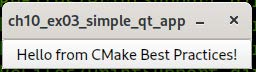
\includegraphics[width=0.3\textwidth]{content/2/chapter10/images/1.jpg}\\
Figure 10.1 – The simple Qt application window
\end{center}

With this sorted out, we have concluded the part that learns about how to use super-build in a CMake project. Next, we will be taking a look at ensuring version consistency in a super-build.

















